\begin{explanationbox}
	\textbf{为什么沿圆心连线找极值？}

	圆周上的所有点离圆心都一样远，均为 $R$。从 $P$ 经 $O$ 到圆周最远端，恰好走一条直线；从 $P$ 朝圆心走，到最近端只需走 $d-R$。偏离这条直线时，三角形三边关系保证距离严格介于二者之间。

	最近端：$P,C,O$ 依次共线，$PC=PO-CO=d-R$。\begin{center}
		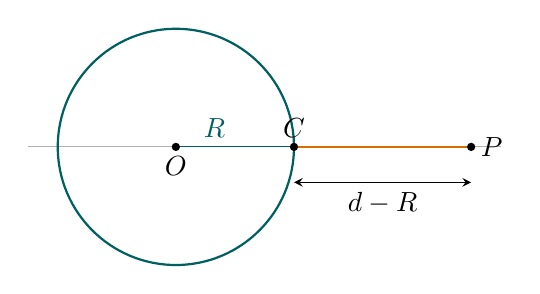
\begin{tikzpicture}[scale=.75,>=stealth]
 \coordinate (O) at (0,0); \coordinate (P) at (5,0);
 \coordinate (A) at (0:2); \coordinate (C) at (2,0); \coordinate (B) at (-2,0);
 \draw[gray!60] (-2.5,0)--(5.5,0);
 \draw[teal!75!black,thick] (O) circle (2);
 \draw[teal!75!black] (O)--(A) node[midway,above left] {$R$};
 \draw[orange!85!black,thick] (P)--(A);
 \fill (O) circle (2pt) node[below] {$O$};
 \fill (P) circle (2pt) node[right] {$P$};
 \fill (C) circle (2pt) node[above] {$C$}; \draw[<->] (2,-.6)--node[below] {$d-R$}(5,-.6);
 \end{tikzpicture}

	\end{center}
	最远端：$P,O,B$ 依次共线，$PB=PO+OB=d+R$。\begin{center}
		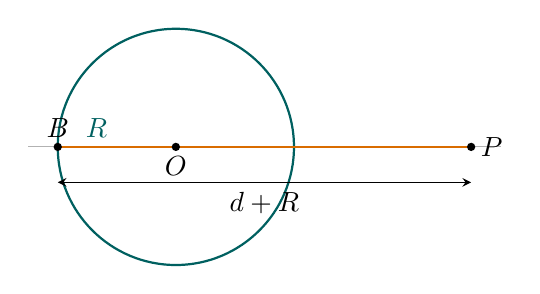
\begin{tikzpicture}[scale=.75,>=stealth]
 \coordinate (O) at (0,0); \coordinate (P) at (5,0);
 \coordinate (A) at (180:2); \coordinate (C) at (2,0); \coordinate (B) at (-2,0);
 \draw[gray!60] (-2.5,0)--(5.5,0);
 \draw[teal!75!black,thick] (O) circle (2);
 \draw[teal!75!black] (O)--(A) node[midway,above left] {$R$};
 \draw[orange!85!black,thick] (P)--(A);
 \fill (O) circle (2pt) node[below] {$O$};
 \fill (P) circle (2pt) node[right] {$P$};
 \fill (B) circle (2pt) node[above] {$B$}; \draw[<->] (-2,-.6)--node[below] {$d+R$}(5,-.6);
 \end{tikzpicture}

	\end{center}
	\textbf{识别信号：} 定点、圆周动点、距离或距离平方的最值。先找圆心与半径，再算圆心距；通常无需求动点坐标。
\end{explanationbox}
